\chapter{Document Control}

\section*{What problem are we trying to solve?}
\begin{marginfigure}
  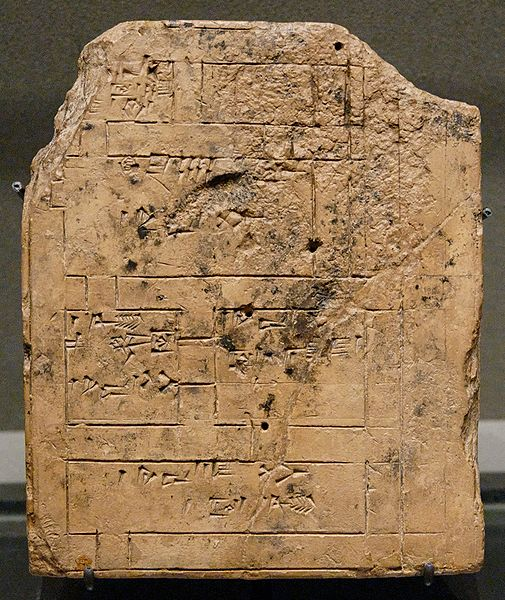
\includegraphics[width=\linewidth]{gudea-plans}
  \caption{Clay plans of a six-room building, a sanctuary or a private house. From Telloh, ancient Girsu circa 2125, from \url{http://en.wikipedia.org/wiki/Gudea_cylinders}}
  \label{fig:marginfig1}
\end{marginfigure}
If you ever lost a document you will agree that there is always a need to keep control of important documents. The document control system has been designed to aid in the  filing of documents and provide an easy way of retrieving this information.
Some documents we keep because is required by law to keep them. Others we need them in order to control the flow of money in a Company. To summarize the system described in this chapter will help you file your documents better and enable you to retrieve these documents easier.

\section*{What is document control?}

Document control means that the right persons have the current version of the documents they need, while unauthorized persons are prevented access to them.

We all handle many documents every day. These documents include forms that we fill out, instructions that we follow, invoices that we enter into the computer system, holiday schedules that we check for the next day off, rate sheet that we use to bill out customers, and many more.

An error on any of these documents could lead to problems. Using an outdated version could lead to problems. Not knowing if we have the latest version or not could lead to problems. And so on.

The Document control system affects our entire company, and all business related documents must be controlled. Only documents that don’t have an impact on our products, services or company don’t need to be controlled – all others need to be controlled. This means, basically, that any business related documents must be controlled. 

\section*{Whose responsibility?}

\begin{marginfigure}
  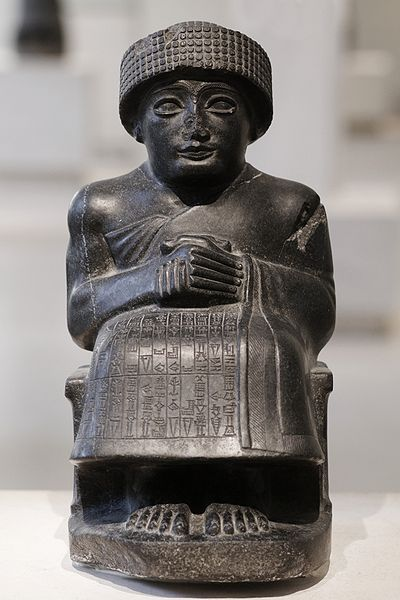
\includegraphics[width=\linewidth]{gudea}
  \caption{Diorite statue od the earliest known document Controller. Mesopotamia circa 2150 BC.}
  \label{fig:marginfig1}
\end{marginfigure}

Document control is the responsibility of all employees. It is important that all employees understand the purpose of document control and the tools (requirements) that help us control our documents.

Please be aware that if you copy a document or print one out and then distribute it, you are responsible for controlling the distribution! The original author won't know that you distributed more of his documents, so the original author can't control that distribution. That is why on critical job sites all copies, faxing and distribution is via our DCC (Document Control Center)






\section*{Project Filing}


\begin{marginfigure}
  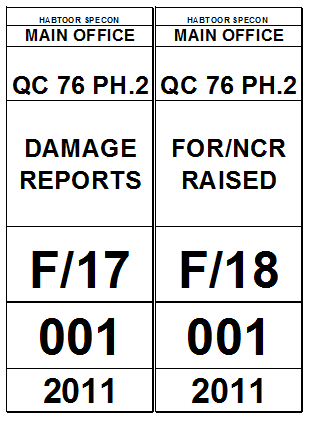
\includegraphics[width=\linewidth]{labels}
  \caption{Typical labels.}
  \label{fig:marginfig1}
\end{marginfigure}

Project filing, follows closely to the system set up at Head Office. You can think of Document Control a bit like the post office where communication is always between one office to another. In many respects filing on sites is more difficult and challenging due to its temporary nature and the changing number of employees as the Project moves through the different phases.

Files are labeled with letters and numbers:

\begin{center}
\fbox{
       \begin{minipage}{6.0cm}
        FILE REF. NO. A/1

        Outgoing Correspondence.
       \end{minipage}
}
\end{center}
        
When files overflow we number them consequentially as follows:

\begin{center}
\fbox{
       \begin{minipage}{6.0cm}
        FILE REF. NO. A/1-001

        Outgoing Correspondence.

        FILE REF. NO. A/1-002

        Outgoing Correspondence.
 \end{minipage}
}
\end{center}

The file references are initially chosen to represent a comprehensive Master File list. An extract from such a Master List is in Table\ref{masterlist}.


\begin{fullwidth}
\begin{table}[htb]
\vspace{0.5cm}

\small
\hskip-10pt\begin{tabular}{|l|l|l|l||l|l||l|l||l|l|l|}
\hline
File &Category        &Control              & Person       &Copy 1  &Person        &Copy 2        &Person      &Copy 3 &Person\\
     &                &Copy location        & resp. &        &resp.   &resp.   &resp. &      &resp.\\
\hline
A/1    & Corresp (in).       & H.O. Sec.           & H.O. Secr. & Site & PM           &              &            &      & \\
A/2    & Corresp.(out)       & H.O. Sec.           & H.O. Secr. & Site & PM           &              &            &      & \\
A/3    & memos (in)          & H.O. Sec.           & H.O. Secr. & Site & PM           &              &            &      & \\
A/4    & memos (out)         & H.O. Sec.           & H.O. Secr. & Site & PM           &              &            &      & \\
\hline
\end{tabular} 	
\caption{Extract from filing list}
\label{masterlist}
\end{table}
\end{fullwidth}

What is important to notice in the Table above, that in many cases the filing system allows for up to three copies to be kept, but there is always a two tier system where there is a \textit{control copy}, normally kept at head office and one or two copies kept at other locations. If the site is far from head office or for cases where there is no need to keep copies at Head Office the Document Control Department always keeps the master copy.

It is also important to note that documents have \textit{owners}. In the extract shown in Table\ref{masterlist}. The owner is the responsible person to make sure that the documents have been filed properly. In most cases this person in the Project Document Controller, but for example for orders the Materials Control Manager is the ultimate responsible person to ensure that MCD documents are filed properly.

\subsection*{Document Order}

In general document are filed by \textit{date order}. Numbered documents such as submittals, Quality Assurance Documents and the like bear that bear \textit{reference numbers} are filed \textit{sequentially}. Accounting documents
such as creditors invoices are filed by \textit{date} in the master file and a second copy by \textit{Creditors name}. By choosing
carefully the method of filing and normally by having two different methods enables retrieval of the document easier. In general if the system
is computerized retrieval becomes easier.  

\section*{Setting up the system}

The filing system should be set at the begining of a new Project. Although this sounds simple and intuitive most Projects start without adequate
space, building shelving as we go and continuously buying files. On a well designed system \textit{all} file categories are set up when the Project starts, they are labelled uniformly. As a rule of thumb the minimum space is that of a 20 foot container - and this assuming that files with multiple volumes are archived at certain points. If you do not give it attention at the beginning of the Project you will literally
drawn in paper work nobody will be able to find anything and  everyone will build their own system as they will not have any \textit{faith} in yours!

The equation below, can be used to estimate the number of files that will be required for a project:



$$ N = \frac{p^{0.8}(t + d)}{d} $$

where,

N = number of files

p = mean personnel on project

t = duration of project (months)

d = number of departments




\section*{When to file}

Generally if people responsible for filing do not clear their intrays daily it leads to problems with retrieval. What happens as they have a continuous backlog the bottom of the tray never gets cleared and after a week or two documents cannot be found (so we get another copy from whoever sent it to us) which leads to another problem that eventually when we find the document we now have two identical copies in the file and 
stamped with two different incoming date stamps.

\section*{Getting the right equipment}

During the two critical \textit{crunch periods} of the Project, which are normally the start and end of the Project you will find that
documents and document copying and processing is at its peak. During this time of the project unless the Site and its partner Companies have a decent photocopier the flow of documents will slow down tremendously. It is not unknown for documents to take 11 days to be delivered from the Consultant's desk (via their own document control) to that of the Main contractors's and then to us. For comparison in 1890 a letter would travel at the cost of 1 penny with the Imperial Penny Post from London to Cape Town by steam ship in less than 20 days and taht was door to door delivery. In general a decent photocopier should be purchased based on expected volumes of copying which should never be less than 20000 copies per month (to keep up with peaks). This should be able to interface with a computer and the network and if you are going to charge subcontractors  departments or Clients it should have a keypad for logging usage. When the latter is not used, it is also not unknown for people to introduce 
manual systems of approval and logging of copies usage introducing another cost to the Company and further contributing to bureacratic bloat, inefficiency and delays. 

\section*{Key performance indicators}

Document Control should be able to produce all necessary log forms weekly by close of business every Thursday or at a date agreed with the Project Director. Normally these are:

\begin{table}
\begin{tabular}{l}
\toprule
Material Submittal logs\\
RFI logs\\
WIR logs\\
\bottomrule
\end{tabular}
\caption{Weekly logs produced by Document Control}
\end{table}


Document Control should be able to retrieve a document within a maximum of 30 minutes and deliver a copy (right? you don't want the original copies to leave Document Control - so you do need a good and fast photocopier). The best performance indicator is for the Document Control Department is to keep it \textit{customers} happy. 

\section*{Dating documents}

Require us to show on every document when it was created or last updated. Many of us thought about using the automatic date field for this but….
Should we use the automatic date field on documents?

Generally not, if you enter the automatic date field into a document, the field will automatically be updated to always show the current date, no matter when you actually created or updated the document.



Another example:

Another example is entering the automatic date field in the footer of a document that you frequently change and then print. You may have used the automatic date field as an easy way to see on your printouts when they were printed; the idea here was that the document with the latest date is the most current printout. However, you may make one printout today and another tomorrow without having made any changes to the document. Though both printouts are identical, they now show different dates. This will inevitably lead to confusion. 

Document control requires us to show on any document when it was created or last updated. The automatic date field is not suitable for this. Therefore, as a general rule, don’t use the automatic date field to identify version status.


\section*{Forms}

Yes, a form must be controlled as long as the form has an impact on our services or our company.

Blank forms are similar to instructions as they guide the user to provide certain information. If the form is outdated or incomplete, the user will not be prompted to supply all the necessary information. It is, therefore, important to control blank forms like any other document.

Once a form is filled out, however, it has become a record. At this point, we need to be concerned with filing, storage, archiving, and eventually destruction.
All forms and documents are specified in the Company ISO Manual.

\section*{Policies and procedures}

While most procedure affect only managers, all employee must be familiar with the \textit{Quality Policy} and with the \textit{Document Control Procedure}.

\section*{Document Control Organization}

The Document control department is actually a Main Department and sattelites. Sattelite sections will exist in other Departments. In general it should be organized as follows:

\begin{verbatim}
- Document Control (Central Department)
-- Administration /HR (visa related, personnel passports, drivers, petrol control)
-- Correspondence (secretary)
-- QA/QC
-- QS
-- Procurement
-- Design (very limited)
-- CAD Office
-- Accounts
-- Stores (own copies of delivery notes, returns issues etc).
-- Safety department
\end{verbatim}

The particular contributions of these departments are laid out in their respective Business process sections. The Document Control department is normally staffed with 3-4 people. The Document Controller, one or two assistants and a person dedicated to photo-copying. 


\section*{Computerized Systems}

Computerized systems do not eliminate the need for paper filing but can reduce it. They can also assist in retrieval and distribution. Unless
your manual system is working well, computerization is next to impossible.


\section*{Archiving and disposal of documents}
\begin{marginfigure}
  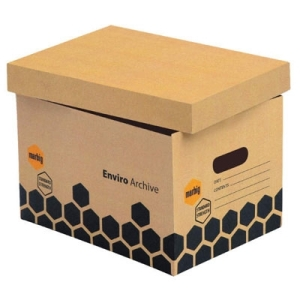
\includegraphics[width=\linewidth]{archivebox}
  \caption{Environmental friendly box}
  \label{fig:marginfig1}
\end{marginfigure}
At the end of the Project most of the items will require to be disposed or archived. Having now contributed considerably to the destruction of the environment by using all this paper and possibly finished a monstrosity on a pristine location, this can be done by buying environmentally friendly boxes made for the purpose. Documents to be disposed should be shredded if possible. If the system has been followed and monitored, this should be a simple operation as all the filing will already be in boxes and what it means is that only the last files will be boxed. Label the boxes accordingly and state the date that the contents can be disposed off.

\section*{Summary}

This short document described some of the issues relating to the control of Company documents. As a last word do some kaizen.\sidenote{\href{Kaizen}{http://en.wikipedia.org/wiki/Kaizen}.}


























